\documentclass[12pt,letterpaper]{article}
\usepackage[spanish]{babel}
\usepackage[left=2cm,top=2cm]{geometry}
\usepackage[utf8]{inputenc}
\usepackage{helvet}
\usepackage{amsmath,amssymb}
\usepackage{enumitem}
\usepackage{pgfplots}
\usepackage{gensymb}
\usepackage{graphicx} 
\usepackage{setspace}
\usepackage[spanish]{babel}
\usepackage[left=2cm,top=2cm]{geometry}
\usepackage[utf8]{inputenc}
\usepackage{colortbl}
\usepackage{setspace}
\usepackage{hyperref}
\usepackage{float}
\onehalfspacing

\usepackage{fancyhdr}	% Para manejar los encabezados y pies de página
\pagestyle{fancy}		% Contenido de los encabezados y pies de pagina
\usepackage{float}		% Para ubicar las tablas y figuras justo después del texto
\usepackage{booktabs}	% Para hacer tablas más estilizadas
\usepackage{multirow}
\onehalfspacing
\usepackage{float}
\usepgfplotslibrary{external}
 \pgfplotsset{width=10cm,compat=1.9}
\selectlanguage{spanish}
\newcommand{\grad}{$^{\circ}$}% Escribir \grad Celcius 

\lhead{Orden Digital} 
\chead{}
\rhead{Web Data}
\lfoot{} 
\cfoot{\thepage}
\rfoot{}

\author{ \textbf{Elaborado por: }Aarón Josué Sibaja Villalobos}
\title{Orden Digital \vspace{2cm}\\
\noindent\rule{13cm}{0.4pt} \\
 \textbf{Web Data}\\
\noindent\rule{13cm}{0.4pt}\\
\vspace{4cm}
 }
\date{\vspace{5cm} Junio, 2017 }
 		

\begin{document}

\maketitle
\thispagestyle{empty}


\newpage
\setcounter{tocdepth}{3}
\tableofcontents
\newpage
\listoffigures

\newpage
\section{Descripción: }

El presente documento detalla  la funcionalidad del proyecto Web Data, cuyo propósito es extraer metadata de las redes sociales asociados a una búsqueda (palabras o conjunto) dada por el usuario. Esto con el propósito de hacer posteriormente una análisis exploratorio o predictivo con los datos. 

El proyecto se encuentra  en el lenguaje de programación \textit{Python}. Esto con el propósito de poder sacar ventaja de sus herramientas para el desarrollo de \textit{Web Minning}.

\section{Consideraciones previas:}
Para hacer uso del correcto del programa se debe de hacer una previa instalación del lenguaje de programación Python. Es preferible hacer uso de una version 2.7.XX correspondiente a su última actualización, esto para garantizar su estabilidad. Se recomienda descargarlo de la página oficial: 
\begin{center}

\url {https://www.python.org/downloads/} 
\end{center}

Seguidamente que se tiene instalado no está de más verificar la instalación y versión de \textit{Python}. Mediante el gestor de paquetes nativo de \textit{Python} \" pip \"se deben de instalar librerías para el manejo de Twitter:

\begin{itemize}
\item pip install tweepy
\item pip install twitterstream

\end{itemize} 


Luego se debe de informar a Twitter que se va a hacer uso de su plataforma, mediante su página oficial de desarrollo Twitter Application Management:

\begin{center}
\url {https://apps.twitter.com/} 
\end{center}

Después de crear una cuenta, se debe crear una nueva aplicación. Hay que insertar, un nombre para la aplicación, una breve descripción y algún website, para este caso se utilizo el repositorio de Github. Lo anterior se hace con el motivo de generar \textit{Key y Access Tokens }, credenciales necesarias para extraer los datos desde Twitter.

\section{Módulos del Proyecto:}

El proyecto se divide en tres partes principales:

\subsection{Data}

Contiene los archivos referentes el manejo de la manipulación de los datos. Se encuentra la opción de guardado a una base de datos MySQL o como salida en un  archivo csv.
\subsection{ Robot}

 Contiene los módulos para crear demonio que se ejecute a conveniencia. Esto con el propósito de establecer intervalos de extracción personalizados dependiendo de las exigencias que se presenten.

\subsection{Twitter} 

Contiene lo códigos para la extracción de los datos en la red social. Contiene las respectivas credenciales configuradas específicamente para la aplicación como se detallo anteriormente.


\appendix
\section{Cronograma}
\begin{figure}[H]
\centering
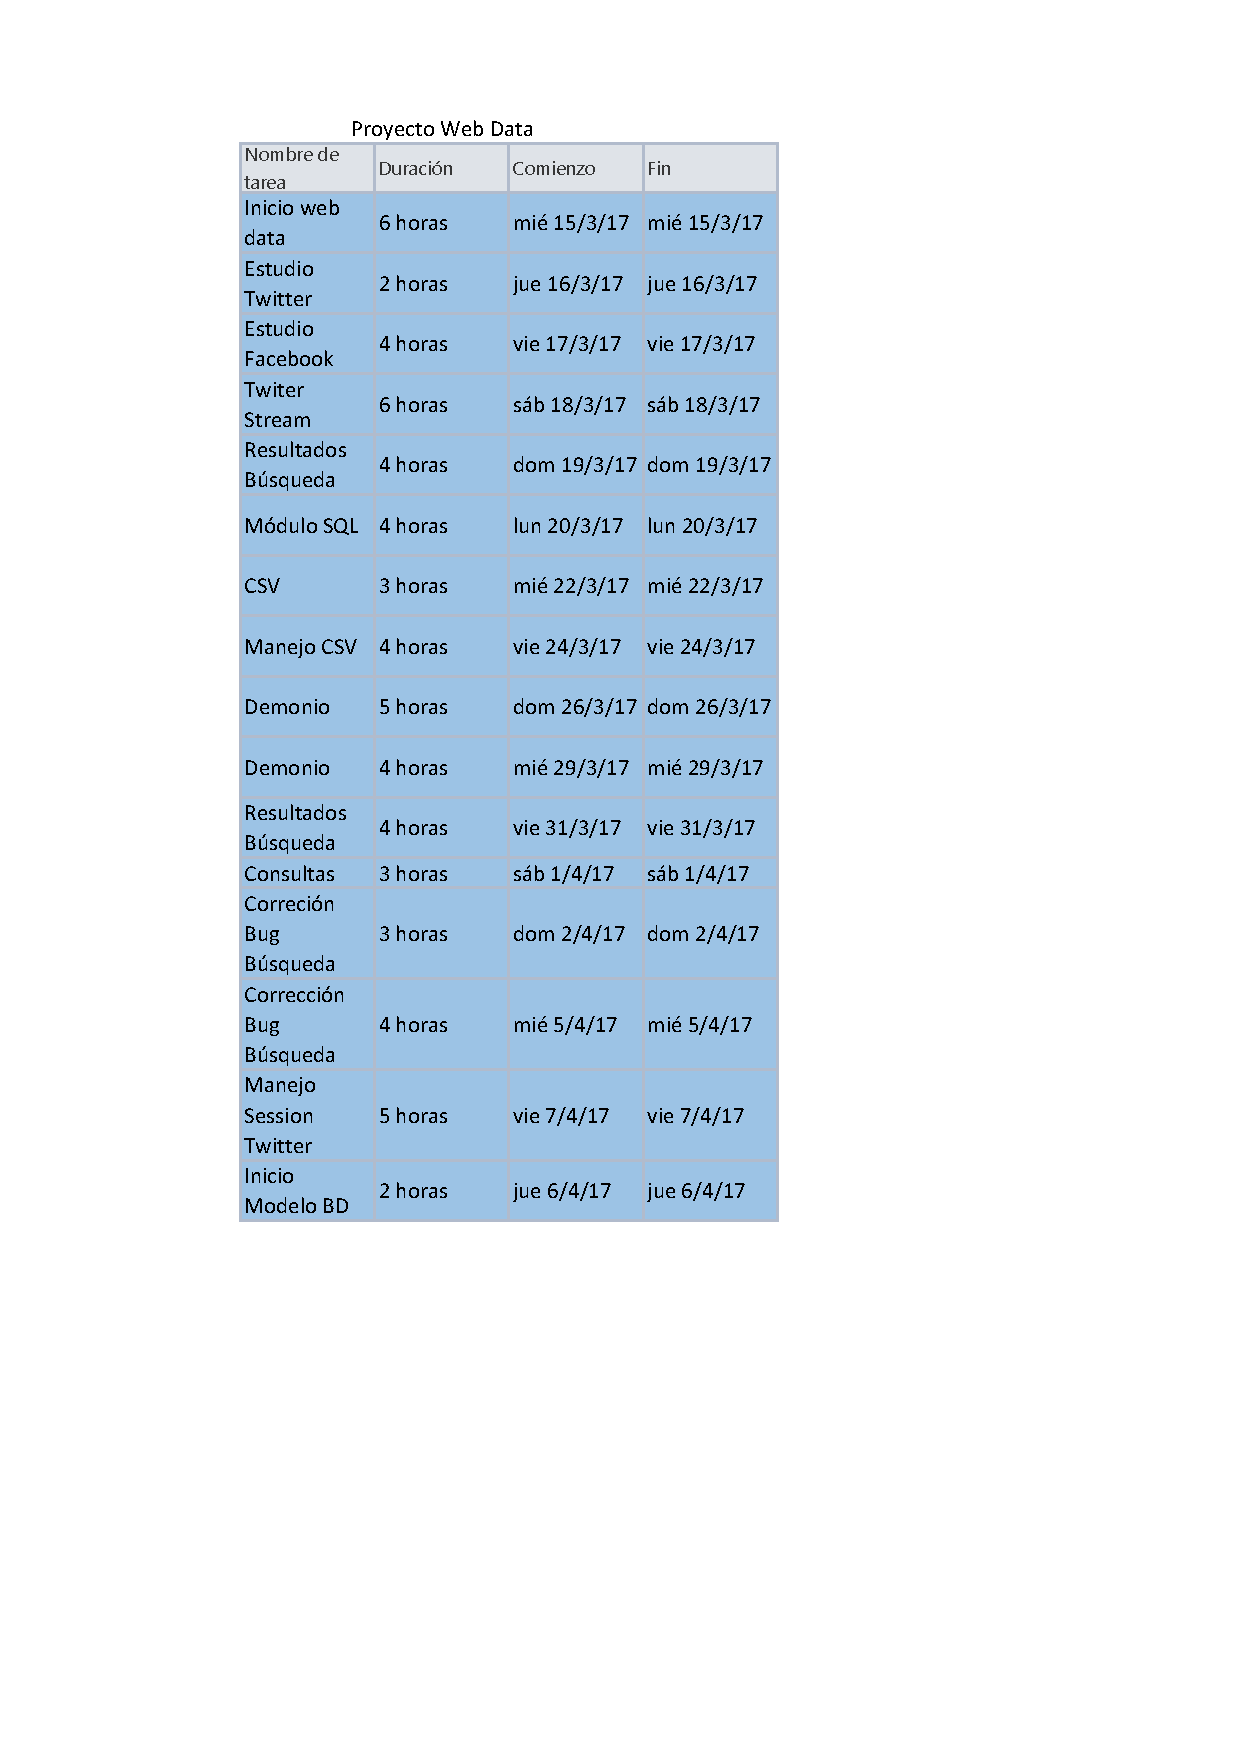
\includegraphics{CronogramaOrdenDigital.pdf}
\caption{Cronograma de Actividades.}
\label{}
\end{figure}

\end{document}
